\chapter{General matrix function approximation}
\label{chap:general_matfunc}

We now consider Krylov subspace methods for approximating \( \fA \vec{v} \) for more general \( f \).
In \cref{sec:lanczos_FA} we discuss the Lanczos method for matrix function approximation (Lanczos-FA), which is probably the most widely used algorithm for this task.
Then, in \cref{sec:lanczos_OR_gen}, we discuss how Lanczos-OR iterates can be used to generate approximations to a wide range of functions.


\section{Explicit polynomial methods}

A simple approach to approximating \( \fA\vec{v} \) is to compute 
\begin{equation*}
    \ff{f}{k-1}\mf{\vec{A}} \vec{v} \in \mathcal{K}_{k}
\end{equation*}
where \( \ff{f}{k-1} \) is some polynomial chosen to approximate \( f \).
For instance, the Chebyshev semi-iterative method mentioned in the example from \cref{chap:intro} falls into this category of algorithms.

If \( |f - \ff{f}{k-1}| \) is not strongly correlated with the eigenvalues of \( \vec{A} \), we might expect 
\begin{equation*}
    \| \fA \vec{v} - \ff{f}{k-1}\mf{\vec{A}} \vec{v} \|
    > c \| f - \ff{f}{k-1} \|_{\mathcal{I}} \| \vec{v} \|
\end{equation*}
for some reasonable constant \( c \).

Like mentioned in our discussion of algorithms for quadratic forms in \cref{sec:QF_tradeoffs}, one nice property of explicit polynomial methods is the lack of inner products, which can be expensive on supercomputers. 
In addition, explicit polynomial methods for \( \fA\vec{v} \) do not require storing a basis for Krylov subspace.

\section{Lanczos-FA}
\label{sec:lanczos_FA}

Early uses of Lanczos-FA were focused primarily on computing matrix exponentials applied to a vector; i.e. \( f = \exp(tx) \).
As far as we can tell, Lanczos-FA was introduced in \cite{nauts_wyatt_83} and first used for general \( f \) in \cite{vandervorst_87}.
Soon after Lanczos-FA was first used, a number of papers studying the algorithm and its convergence properties were published \cite{park_light_86,druskin_knizhnerman_88,druskin_knizhnerman_89,gallopoulos_saad_92,saad_92}.
These early works were followed by a number of papers demonstrating the effectiveness of Lanczos-FA in finite precision arithmetic \cite{druskin_knizhnerman_91,druskin_knizhnerman_95,druskin_greenbaum_knizhnerman_98}, a topic we discuss further in \cref{chap:finite_precision}.


\begin{definition}
    \label{def:lanczos_fa}
The \( k \)-th Lanczos-FA approximation to \( f\A\vec{v} \) is
\begin{equation*}
    \lan_k(f) 
    := \vec{Q} f\mf{\vec{T}} \vec{e}_0.
\end{equation*}
\end{definition}

\begin{remark}
\label{rem:CG_MINRES}
If \( \vec{A} \) is positive definite, then the Lanczos-FA approximation to \( f = 1/x \) coincides with the CG iterate defined in \cref{sec:linear_solvers}.
 Even when $\vec{A}$ is indefinite, we can use the Lanczos-FA iterate as an approximation to \( \vec{A}^{-1}\vec{v} \).
However, the resulting algorithm is not guaranteed to be optimal, and if $\vec{T}$ has an eigenvalue near to or at zero then $\vec{T}^{-1}$ will be poorly conditioned or even undefined. 
Even so, the \emph{overall} convergence of the Lanczos-FA iterate is closely related to the convergence of MINRES.
    We described this phenomenon in detail in \cref{sec:CG_indefinite}. \qedhere
\end{remark}


A basic property of the Lanczos-FA iterate is that polynomials are applied exactly. 
More precisely, we have the following, well known, theorem.
\begin{theorem}
    \label{thm:lanczosFA_exact}
    Suppose \( \deg(p) < k \). 
    Then,
    \begin{equation*}
        \lan_k(p) = \pA \vec{v}.
    \end{equation*}
\end{theorem}

\begin{proof}
    Using \cref{thm:tridiag_power} we have
    \begin{align*}
        \vec{A}^{q} \vec{v} = \vec{A}^q \Qhat \vec{e}_0
        = \Qhat \widehat{\vec{T}}^q \vec{e}_0
        = \vec{Q} \vec{T}^q \vec{e}_0.
    \end{align*}
\end{proof}


This theorem implies that, when \( \mu = \Psi \), 
\begin{equation*}
    \lan_k(f) = \ff[i]{f}{k-1}\mf{\vec{A}} \vec{v}.
\end{equation*}
In other words, the Lanczos-FA iterate is obtained by interpolating \( f \) at the eigenvalues of \( \vec{T} \) with a degree \( k-1 \) polynomial.



\subsection{A priori error bounds on an interval}

Akin to the bounds we saw in \cref{sec:quadrature_apriori}, we can derive a bound based on best approximation on an interval.
\begin{theorem}
\label{thm:poly_unif}
    The Lanczos-FA iterate satisfies
\begin{equation*}
    \frac{\| \fA \vec{v} - \lan_k(f) \|}{\|\vec{v}\|}
    %&\leq  2 \left( \min_{\deg(p)<k} \max_{x \in \mathcal{I}\A} | f(x) - p(x) | \right) \| \vec{v} \|_2.
    \leq  2 \min_{\deg(p)<k} \| f-p \|_{\mathcal{I}} .
\end{equation*}   
\end{theorem}
\begin{proof}
For any polynomial \( p \) with \( \deg(p) < k \),
\begin{align*}
\| \fA \vec{v} - \lan_k(f) \|
& \leq \| \fA \vec{v} - \pA \vec{v} \| + \| \lan_k (p) - \lan_k (f) \| 
\\& = \| (\fA - \pA )\vec{v} \| + \| \vec{Q} ( p\mf{\vec{T}} - f\mf{\vec{T}} ) \vec{Q}^{\cT} \vec{v} \| 
\\& \le \| \fA - \pA \|_2  \| \vec{v} \| + \| \vec{Q} ( p\mf{\vec{T}} - f\mf{\vec{T}} ) \vec{Q}^{\cT} \|_2  \|\vec{v} \|
\\& \le ( \| \fA - \pA \|_2 + \| p(\vec{T} ) - f\mf{\vec{T}} \|_2 )  \| \vec{v} \| . 
    \\& = ( \| f-p \|_{\Lambda} + \| f-p \|_{\Lambda\mf{\vec{T}}} )  \| \vec{v} \| . 
\end{align*}
Then, optimizing over polynomials of degree less than \( k \),
\begin{equation}
\| \fA \vec{v} - \lan_k(f) \|
    \leq \min_{\deg(p)< k} \left( \| f-p \|_{\Lambda} + \| f - p \|_{\Lambda\mf{\vec{T}}} \right) \| \vec{v} \|. \label[ineq]{eqn:triangle_ineq1}
\end{equation}
Finally, using that \( \Lambda,\Lambda\mf{\vec{T}} \subset \mathcal{I} \), we obtain the result.
\end{proof}

As we will discuss in \cref{chap:finite_precision}, bounds for Lanczos-FA based on polynomial approximation on \( \mathcal{I} \) still hold, to close approximation, in finite precision arithmetic.

%\Cref{thm:poly_unif} asserts that, except for a possible factor of \( 2 \), the error of the Lanczos-FA approximation to \( \fA \vec{v} \) is at least as good as the best polynomial approximation to \( f \) on the interval containing the eigenvalues of \( \vec{A} \).
%For arbitrary \( f \), \cref{thm:poly_unif} remains the standard bound for Lanczos-FA. 
%As we discuss in \cref{chap:finiite_precision}, it has been studied carefully and is known to hold to a close degree in finite precision arithmetic \cite{musco_musco_sidford_18}.
%However, as we have noted throughout this thesis, such bounds are insufficient to truly describe the behavior of many methods, including Lanczos-FA.

\subsection{Two-pass Lanczos-FA}

A major downside of Lanczos-FA compared with explicit polynomial approaches is that a simple implementation requires that \( \vec{Q} \) be stored.
Fortunately, this storage cost can be avoided by incurring additional computational cost. 
In particular, we can use an implementation called two pass Lanczos-FA \cite{boricci_00a,frommer_simoncini_08}.
On the first pass, the tridiagonal matrix $\vec{T}$ is computed using the short-recurrence version of Lanczos; i.e., without storing all of $\vec{Q}$.
Once $\vec{T}$ has been computed, $f(\vec{T}) \vec{e}_0$ can be evaluated using $O(k^2)$ storage.
Lanczos is then run again and the product $\vec{Q} f(\vec{T}) \vec{e}_0$ is computed as the columns of $\vec{Q}$ become available.
Note that on the second run, the \emph{exact same} Lanczos vectors (even in finite precision arithmetic) can be computed without any inner products by using the values computed in the first run and stored in \( \vec{T} \).


Such an approach can be generalized by re-generating the Lanczos recurrence from multiple points simultaneously on the second pass \cite{li_22}.
Specifically, on the first pass, vectors \( \vec{q}_j \) and \( \vec{q}_{j-1} \) can be saved for \( j=0,d,2d,\ldots \). 
Then, on the second pass, the rest of the Lanczos vectors can be constructed by continuing the three-term Lanczos recurrence \cref{eqn:lanczos_three_term} from each of the roughly \( n/d \) start points in parallel. 
Thus, the number of matrix-loads is reduced by a factor of roughly \( d \) at the cost of storing roughly \( 2n/d \) vectors.
The case \( d=n \) gives the original two-pass approach.

\section{Lanczos-OR based methods}
\label{sec:lanczos_OR_gen}

\iffalse
As an alternate motivation for the Lanczos-FA iterate, we note that many functions can be written in the form
\begin{equation*}
    f(x) = \int_{\Gamma} \frac{g(z)}{x-z} \d{z}
\end{equation*}
for some contour \( \Gamma \) and function \( g \).
Indeed, such functions include Stieltjes functions, analytic functions, and rational functions.
In such cases, it is not hard to see that
\begin{equation*}
    \fA \vec{v} = \int_{\Gamma} g(z) (\vec{A} - z\vec{I})^{-1} \vec{v} \d{z}.
\end{equation*}
As discussed in \cref{rem:CG_MINRES} and justified in \cref{sec:CG_MINRES}, for a fixed value \( z\in\mathbb{C} \), we can approximate \( (\vec{A} - z\vec{I})^{-1} \vec{v} \) by means of the formal expression for the conjugate gradient algorithm; i.e. by 
\begin{equation*}
    (\vec{A} - z\vec{I})^{-1} \vec{v} \approx \vec{Q} (\vec{T} - z\vec{I})^{-1} \vec{e}_0.
\end{equation*}
Integrating the resulting approximation we obtain
\begin{equation*}
    \int_{\Gamma} g(z) \vec{Q} (\vec{T} - z\vec{I})^{-1} \vec{e}_0 = \vec{Q} f\mf{\vec{T}} \vec{e}_0 = \lan_k(f).
\end{equation*}
We will use the integral representation to derive error bounds for Lanczos-FA in \cref{chap:CIF}.

\fi

We can use integral representations of functions to derive algorithms based on Lanczos-OR iterates.
For concreteness, we consider the case of the matrix-sign function and rational functions in partial fraction form.
It's clear that a similar approach can be applied to other functions, and further study of the resulting algorithms would be interesting.


\subsection{The matrix sign function}
\label{sec:sign_function}

We begin by noting that, for any $a>0$,
\begin{equation*}
    \frac{1}{\sqrt{a}}
    = \frac{2}{\pi} \int_0^\infty \frac{1}{a + z^2} \d{z}.
\end{equation*}
%\Anne{[Is it standard to write this as $\frac{1}{\sqrt{x^2}}$ instead of  $\frac{1}{|x|}$?]}
Thus, if $f = \operatorname{sign}=x/|x| = x/\sqrt{x^2}$, we have 
\begin{equation*}
    \fA\vec{v} = \frac{2}{\pi} \int_0^\infty  \vec{A}(\vec{A}^2 + z^2\vec{I})^{-1} \vec{v} \: \d{z}.
\end{equation*}
The Lanczos-OR approximation to $\vec{A}(\vec{A}^2 + z^2\vec{I})^{-1} \vec{v}$ is $\vec{Q} ([\widehat{\vec{T}}^2]_{:k,:k} + z^2\vec{I})^{-1} \vec{T} \vec{e}_0$, which is optimal over Krylov subspace in the $(\vec{A}^2 + z^2\vec{I})$-norm.
This yields the approximation 
\begin{equation*}
    \frac{2}{\pi} \int_0^\infty \vec{Q} ([\widehat{\vec{T}}^2]_{:k,:k} + z^2\vec{I})^{-1} \vec{T} \vec{e}_0 \: \d{z}
    = \vec{Q} \left([\widehat{\vec{T}}^2]_{:k,:k} \right)^{-1/2} \vec{T}  \vec{e}_0.
\end{equation*}
Thus, we can define the induced iterate as
\begin{equation}
    \label{def:sign_or}
\mathsf{sign-OR}_k := \vec{Q} \left([\widehat{\vec{T}}^2]_{:k,:k} \right)^{-1/2} \vec{T}  \vec{e}_0
=
\vec{Q} \left( [\widehat{\vec{T}}]_{:k,:k+1}[\widehat{\vec{T}}]_{:k+1,:k} \right)^{-1/2} \vec{T}  \vec{e}_0.
\end{equation}


\subsubsection{Relation to Lanczos-FA}

The Lanczos-OR and Lanczos-FA iterates for a given rational matrix function are clearly related. 
In particular, $\tilde{N}\mf{\vec{T}}$ and $[\tilde{N}(\widehat{\vec{T}})]_{:k,:k}$ differ only in the bottom rightmost $(q-1)\times (q-1)$ principle submatrix, where $q = \deg(\tilde{N})$.
Using this fact, it can be shown that the Lanczos-OR and Lanczos-FA iterates ``tend to coalesce as convergence takes place'' \cite[Proposition 5.1]{lopez_simoncini_06}.
We now show that a similar phenomenon occurs with the induced Lanczos-OR approximation to the sign function and the Lanczos-FA approximation.

\begin{theorem}
\label{thm:sign_approx_compare}
The Lanczos-FA and induced Lanczos-OR approximations to the matrix sign function satisfy
\begin{equation*}
    \| \lan_k(\operatorname{sign}) - \mathsf{sign-OR}_k \|_2
    \leq
    \beta_{k-1}^2 
    \frac{\sqrt{\alpha_0^2+\beta_0^2}}{2 \sigma_{\textup{min}}\mf{\vec{T}}^3}.
\end{equation*}
where $\sigma_{\textup{max}}\mf{\vec{T}}$ and $\sigma_{\textup{min}}\mf{\vec{T}}$ are the largest and smallest singular values of $\vec{T}$ respectively.
\end{theorem}


\begin{proof}%[Proof of \cref{thm:sign_approx_compare}]
Let ${N} = x^2 + z^2$ and ${M} = x$.
Note that ${N}\mf{\vec{T}} = [{N}(\widehat{\vec{T}})]_{:k,:k} - \beta_{k-1}^2 \vec{e}_{k-1}\vec{e}_{k-1}^\cT$ so,
\begin{equation*}
    {M}\mf{\vec{T}} \vec{e}_0
%    = {N}\mf{\vec{T}} {N}\mf{\vec{T}} ^{-1} {M}\mf{\vec{T}} \vec{e}_0
    = ([{N}(\widehat{\vec{T}})]_{:k,:k} - \beta_{k-1}^2 \vec{e}_{k-1}\vec{e}_{k-1}^\cT){N}\mf{\vec{T}}^{-1} {M}\mf{\vec{T}} \vec{e}_0.
\end{equation*}
    Thus, rearranging terms and multiplying by $([{N}\mf{\widehat{\vec{T}}}]_{:k,:k})^{-1}$ we find that
\begin{align*}
    &{N}\mf{\vec{T}}^{-1} {M}\mf{\vec{T}} \vec{e}_0 - ([{N}(\widehat{\vec{T}})]_{:k,:k})^{-1} {M}\mf{\vec{T}} \vec{e}_0
    \\&\hspace{6em}= \beta_{k-1}^2 ([{N}(\widehat{\vec{T}})]_{:k,:k})^{-1} \vec{e}_{k-1}\vec{e}_{k-1}^\cT {N}\mf{\vec{T}}^{-1}{M}\mf{\vec{T}} \vec{e}_0
\end{align*}
After left multiplying with $\vec{Q}$, this implies that
\begin{equation*}
    \lan_k(r) - \lanopt_k(r,1)
    = \beta_{k-1}^2 \vec{Q} ([{N}(\widehat{\vec{T}})]_{:k,:k})^{-1} \vec{e}_{k-1}\vec{e}_{k-1}^\cT  {N}\mf{\vec{T}}^{-1}{M}\mf{\vec{T}} \vec{e}_0.
\end{equation*}
Now, suppose that $f = \operatorname{sign}$ and set $ \mathsf{diff}_k := \lan_k(\operatorname{sign}) - \mathsf{sign-OR}_k$ as above.
Then, since the Lanczos-FA approximation can also be induced by an integral over $z\in[0,\infty)$, we have that,
\begin{equation*}
    \mathsf{diff}_k
    = \beta_{k-1}^2 
    \frac{2 }{\pi} \int_{0}^{\infty}
    \vec{Q} ([\widehat{\vec{T}}^2]_{:k,:k} + z^2 \vec{I})^{-1} \vec{e}_{k-1}\vec{e}_{k-1}^\cT (\vec{T}^2 + z^2 \vec{I})^{-1} \vec{T} \vec{e}_0 
    \d{z}.
\end{equation*}
Note that $[\widehat{\vec{T}}^2]_{:k,:k} - \vec{T}^2 = \beta_{k-1}^2 \vec{e}_{k-1} \vec{e}_{k-1}^\cT$ is positive semidefinite.
Therefore, using that $\sigma_{\textup{min}}([\widehat{\vec{T}}^2]_{:k,:k}) \geq \sigma_{\textup{min}}(\vec{T}^2) = \sigma_{\textup{min}}\mf{\vec{T}}^2$,
\begin{align*}
    \| \mathsf{diff}_k \|_2
    &
    = \beta_{k-1}^2 
     \bigg\| \vec{Q} \bigg( \frac{2 }{\pi} \int_{0}^{\infty}
    ([\widehat{\vec{T}}^2]_{:k,:k} + z^2 \vec{I})^{-1} \vec{e}_{k-1}\vec{e}_{k-1}^\cT (\vec{T}^2 + z^2 \vec{I})^{-1} \d{z} \bigg)  \vec{T} \vec{e}_0 
     \bigg\|_2
    \\&
    \leq \beta_{k-1}^2 
     \bigg( \frac{2 }{\pi} \int_{0}^{\infty}
    \| ([\widehat{\vec{T}}^2]_{:k,:k} + z^2 \vec{I})^{-1} \|_2 \| (\vec{T}^2 + z^2 \vec{I})^{-1} \|_2 \d{z} \bigg)  \| \vec{T}\vec{e}_0 \|_2
    \\& \leq
    \beta_{k-1}^2 
     \bigg( \frac{2 }{\pi} \int_{0}^{\infty}
    | (\sigma_{\textup{min}}\mf{\vec{T}}^2 + z^2 )^{-1} |~ | (\sigma_{\textup{min}}\mf{\vec{T}}^2 + z^2 )^{-1} | \d{z} \bigg)  \sqrt{\alpha_0^2+\beta_0^2}
    \\&= \beta_{k-1}^2 
    \frac{\sqrt{\alpha_0^2+\beta_0^2}}{2 \sigma_{\textup{min}}\mf{\vec{T}}^3}.
    \tag*{\qedhere}
\end{align*}
\end{proof}

Since $|\beta_{k-1}|$ tends to decrease as the Lanczos method converges, this seemingly implies that the induced Lanczos-OR iterate and the Lanczos-FA iterate tend to converge in this limit.
However, recall that $\vec{T} = [\widehat{\vec{T}}]_{:k,:k}$ changes at each iteration $k$.
In particular, there is the difficulty that $\vec{T}$ may have an eigenvalue near zero, in which case the preceding bound could be useless.

It is known that \( \vec{T} \) cannot have small eigenvalues in two consecutive iterations, provided the eigenvalues of \( \vec{A} \) are not small \cite{greenbaum_druskin_knizhnerman_99}, a result we will recall in \cref{thm:Tk_invertible_bd}.
Since $\beta_{k-1}$ has little to do with the minimum magnitude eigenvalue of $\vec{T}$ (recall that the Lanczos recurrence is shift invariant), we expect that the ``overall'' convergence of the induced Lanczos-OR iterate and the Lanczos-FA iterate will be similar as Lanczos converges.


\subsection{Rational function approximation}
\label{sec:rational_func}


We can use a similar approach to derive (non-optimal) approximations to rational matrix functions $r(\vec{A})\vec{b}$. 
In many settings, particularly when the rational function $r$ is used as a proxy for a function $f$, this approach is more natural than computing the Lanczos-OR approximation to the rational function directly.
The convergence of such methods is closely related to the quality of the (scalar) rational function approximation as well as the quality of the approximation to the rational matrix function.
Specifically, for any output $\mathsf{alg}(r)$ meant to approximate $r(\vec{A})\vec{b}$, we have the following bound:
\begin{align}
\| f(\vec{A}) \vec{b} - \mathsf{alg}(r) \|
&\leq 
\nonumber
\| f(\vec{A}) \vec{b} - r(\vec{A}) \vec{b} \| +  \| r(\vec{A}) \vec{b} - \mathsf{alg}(r) \|
\\&\leq \nonumber
\| f(\vec{A}) - r(\vec{A}) \|_2 \|\vec{b} \| +  \| r(\vec{A}) \vec{b} - \mathsf{alg}(r) \|
\\&\leq \nonumber
\|\vec{b}\|  \max_{\lambda \in \Lambda} | f(\lambda) - r(\lambda) | +  \| r(\vec{A}) \vec{b} - \mathsf{alg}(r) \|
\\& \leq \underbrace{\|\vec{b}\|  \max_{\lambda \in \mathcal{I}} | f(\lambda) - r(\lambda) |}_{\text{approximation error}} 
    + \underbrace{\vphantom{\max_{\lambda\in\mathcal{I}}}\| r(\vec{A}) \vec{b} - \mathsf{alg}(r) \|}_{\text{application error}}.
    \label{eqn:triangle_ineq}
\end{align}
In many cases, very good or even optimal scalar rational function approximations to a given function on a single interval are known or can be easily computed. 
Thus, the approximation error term can typically be made small with a rational function of relatively low degree \cite{trefethen_19,nakatsukasa_sete_trefethen_18}.

Of course, this bound is only meaningful if the approximation error term is small relative to the application error.
Indeed, we also have
\begin{align}
\| f(\vec{A}) \vec{b} - \mathsf{alg}(r) \|
&\geq 
\big| \| f(\vec{A}) \vec{b} - r(\vec{A}) \vec{b} \| -  \| r(\vec{A}) \vec{b} - \mathsf{alg}(r) \| \big|.
\label{eqn:reverse_triangle_ineq}
\end{align}
This shows that the size of $\| f(\vec{A}) \vec{b} - \mathsf{alg}(r) \|$ is rouhgly the size of $\| f(\vec{A}) \vec{b} - r(\vec{A}) \vec{b} \|$ when $\mathsf{alg}(r)$ is a good approximation to $r(\vec{A}) \vec{b}$.


As we noted, rational function approximations commonly are obtained by discretizing an integral representation using a numerical quadrature approximation. 
For instance, the matrix sign function may be approximated as 
\begin{equation}
    \label{eqn:rational_func}
    r_q\A\vec{v} = \sum_{i=0}^{q-1} \omega_i \vec{A} (\vec{A}^2 + z_i^2 \vec{I})^{-1} \vec{v}
\end{equation}
where $z_i$ and $\omega_i$ are appropriately chosen quadrature nodes and weights \cite{hale_higham_trefethen_08}.

We can of course write $r_q = M_q / N_q$, so it's tempting to set $R_q = 1$ and $\vec{H}_q = N_q\A$ and then use Lanczos-OR to compute the $\vec{H}_q$-norm optimal approximation. 
However, while $r_q$ is convergent to $f$ as $q\to\infty$, $N_q := \prod_{i=0}^{q-1} (x^2
+ z_i^2 )$ is not convergent to any fixed function.
In fact $N_q$ will increase in degree and $\vec{H}_q$ will be increasingly poorly conditioned.
This presents a numerical difficulty in computing the Lanczos-OR iterate in this limit.
More importantly, it is not clear that it is meaningful to approximate a function in this way. 
Indeed, it seems reasonable to expect that, for fixed $k$, as $q\to\infty$,  our approximation should be convergent to something. 
However, we cannot guarantee $\lanopt_k(M_q,N_q)$ is convergent in this limit.

On the other hand, akin to our approach for approximating the integral described in the previous subsection, we can compute the \emph{term-wise optimal} approximations to each term in the sum representation of $r_q$ and output
\begin{equation*}
    \sum_{i=0}^{q-1} \omega_i \vec{Q} ([\widehat{\vec{T}}^2]_{:k,:k} + z_i^2\vec{I})^{-1} \vec{T} \vec{e}_0.
\end{equation*}
In this case, as $q\to\infty$, the approximation is convergent to the integral output. 
It would be interesting to understand when a term-wise optimal approximation behaves nearly optimally.


\section{Numerical experiments}
\label{sec:comparison}


\subsection{The matrix sign function}

We now provide several examples which illustrate various aspects of the convergence properties of Lanczos-OR and Lanczos-OR based algorithms, and show when these new methods can outperform more standard techniques like the classic Lanczos-FA.

As we noted in \cref{sec:sign_function}, Lanczos-OR can be used to obtain an approximation to the matrix sign function. 
A related approach, which interpolates the sign function at the so called ``harmonic Ritz values'', is described in \cite[Section 4.3]{eshof_frommer_lippert_schilling_van_der_vorst_02}.
The harmonic Ritz values are characterized by the generalized eigenvalue problem
\begin{equation*}
     [\widehat{\vec{T}}^2]_{:k,:k} \vec{y} = \theta \vec{T} \vec{y}
\end{equation*}
and are closely related to MINRES in the sense that MINRES produces a polynomial interpolating $1/x$ at the harmonic Ritz values \cite{paige_parlett_vandervorst_95}.
Finally, a standard approach is using Lanczos-FA (or equivalently, Gaussian quadrature) as described in \cref{chap:QF,chap:random_quadrature}.


\subsubsection{Spectrum approximation}

In this example, we show the spectrum approximations induced by the algorithms described above.
We now set $\vec{A}$ to be a diagonal matrix with $1000$ eigenvalues set to the quantiles of a Chi-squared distribution with parameters $\alpha=1$ and $\beta=10$. 
We set $k=10$ and consider approximations to the function $c\mapsto \vec{v}^\cT \bOne [\vec{A} \leq c] \vec{v}$ for a range of values $c$. 
Here $\bOne[x\leq c] = (1-\operatorname{sign}(x-c))/2$ is one if $x\leq c$ and zero otherwise.
We pick $\vec{v}$ as a unit vector with equal projection onto each eigencomponent so that $\vec{v}^\cT \bOne [\vec{A} \leq c] \vec{v}$ gives the fraction of eigenvalues of $\vec{A}$ below $c$.
In the $n\to\infty$ limit, this function will converge pointwise to the cumulative distribution of a Chi-squared random distribution with parameters $\alpha=1$ and $\beta=10$. 
The results are shown in \cref{fig:ch6_sign_spec}.

Note that the Lanczos-FA based approach is piecewise constant with jumps at each eigenvalue of $\vec{T}$.
On the other hand, the harmonic Ritz value and Lanczos-OR based approaches produce continuous approximations to the spectrum.
In this particular example, the spectrum of $\vec{A}$ is near to a smooth limiting density, so the harmonic Ritz value and Lanczos-OR based approaches seem to produce better approximations.
Note that these approximations differ from the KPM approximations in \cref{chap:random_quadrature} in that, like Gaussian quadrature, they adapt automatically to the spectrum of \( \vec{A} \).


We note that it is not typically possible to pick $\vec{v}$ with equal projection onto each eigencomponent since the eigenvectors of $\vec{A}$ are unknown. 
However, by choosing $\vec{v}$ from a suitable distribution, it can be guaranteed that $\vec{v}$ has roughly equal projection onto each eigencomponent.
This is discussed thoroughly in \cref{chap:random_quadrature}.


\begin{figure}[ht]
    \begin{center}
        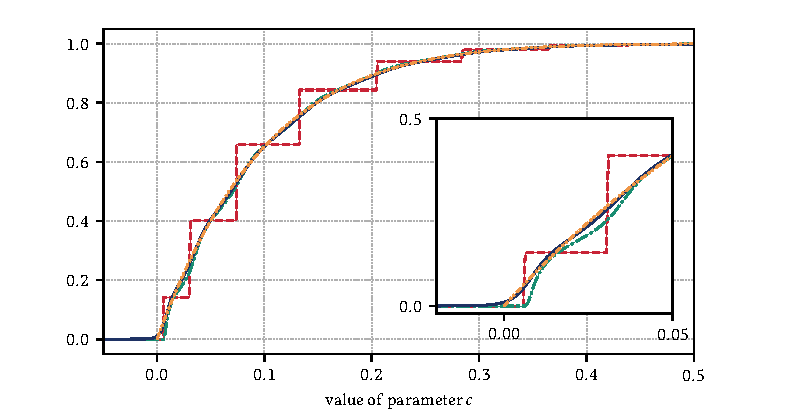
\includegraphics{imgs/ch6_sign_spec.pdf} 
    \end{center}
    \caption[{Comparison of Lanczos-based spectrum approximation algorithms.}]{%
    Comparison of Lanczos-based spectrum approximation algorithms.
    \hspace{.25em}\textit{Legend}:
    Lanczos-OR induced approximation
    ({\protect\raisebox{0mm}{\protect
\includegraphics[]{imgs/legend/l1nm.pdf}}}), 
    Lanczos-FA (GQ) ({\protect\raisebox{0mm}{\protect
\includegraphics[]{imgs/legend/l2nm.pdf}}}),
    harmonic Ritz values based approximation
    ({\protect\raisebox{0mm}{\protect
\includegraphics[]{imgs/legend/l3nm.pdf}}}), and
    limiting density
    ({\protect\raisebox{0mm}{\protect
\includegraphics[]{imgs/legend/l4nm.pdf}}}).
    \hspace{.25em}\emph{Takeaway}: The Lancos-OR and harmonic Ritz value based approximations produce smooth approximations to the spectral density.
    }
    \label{fig:ch6_sign_spec}
\end{figure}

\subsubsection{Quality of approximation}

We now study how the number of matrix vector products impact the quality of approximation for a fixed sign function.

We construct a matrix with $400$ eigenvalues, 100 of which are the negatives of the values of a model problem \cref{eqn:model_problem} with parameters $\kappa = 10^2$, $\rho=0.9$, and $n=100$ and 300 of which are the values of a model problem with parameters $\kappa = 10^3$, $\rho=0.8$, $n=300$.
We then compute the Lanczos-OR induced approximation, the Lanczos-FA approximation, the harmonic Ritz value based approximation from \cite{eshof_frommer_lippert_schilling_van_der_vorst_02}, and the optimal $\vec{A}^2$-norm approximation to the matrix sign function.
The results are shown in \cref{fig:ch6_sign}.
In all cases, we use the Lanczos algorithm with full reorthogonalization.
Because eigenvalues of $\vec{T}$ may be near to zero, Lanczos-FA exhibits oscillatory behavior
On the other hand, the Lanczos-OR based approach and the harmonic Ritz value based approach have much smoother convergence.
Note that the Lanczos-OR induced approximation is not optimal, although it seems to perform close to optimally after a few iterations.

\begin{figure}[ht]
    \begin{center}
        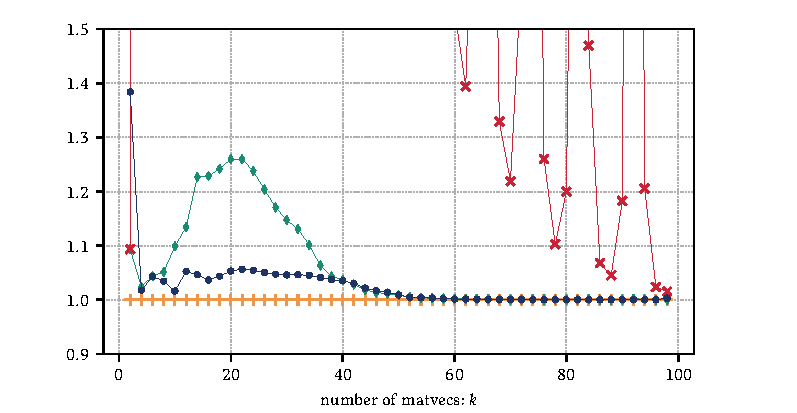
\includegraphics{imgs/ch6_sign.pdf} 
    \end{center}
    \caption[{Optimality ratio for $\vec{A}^2$-norm errors for approximating $\operatorname{sign}\A\vec{v}$.}]{%
    Optimality ratio for $\vec{A}^2$-norm errors for approximating $\operatorname{sign}\A\vec{v}$.
    \hspace{.25em}\textit{Legend}:
    Lanczos-OR induced approximation
    ({\protect\raisebox{0mm}{\protect
\includegraphics[]{imgs/legend/l1.pdf}}}), 
    Lanczos-FA (GQ) ({\protect\raisebox{0mm}{\protect
\includegraphics[]{imgs/legend/l2.pdf}}}),
    harmonic Ritz values based approximation
    ({\protect\raisebox{0mm}{\protect
\includegraphics[]{imgs/legend/l3.pdf}}})
    optimal
    ({\protect\raisebox{0mm}{\protect
\includegraphics[]{imgs/legend/l4.pdf}}}). 
    \hspace{.25em}\textit{Takeaway}: The Lanczos-OR induced approximation to the matrix sign function performs well.
    }
    \label{fig:ch6_sign}
\end{figure}



\subsection{Rational matrix functions}

We now illustrate the effectiveness of the Lanczos-OR based approach to approximating rational matrix functions described in \cref{sec:rational_func}.


\subsubsection{Sign function}

In this example, we use the same spectrum as in the first example.
However, rather than approximating the sign function directly, we instead use Lanczos-OR to approximate each term of a proxy rational function of the form \cref{eqn:rat_form}.
In particular, we consider the best uniform approximation\footnote{Note that the eigenvalues of $\vec{A}$ live in $[-10^2,-1]\cup[1,10^3]$, so we could have used an asymmetric approximation to the sign function.
This would reduce the degree of the rational function required to obtain an approximation of given accuracy, but the qualitative behavior of Lanczos-OR-lm would not change substantially.} of degree $(39,40)$ to the sign function on $[-10^3,1]\cup[1,10^3]$.
Such an approximation is due to Zolotarev \cite{zolotarev_77}, an can be derived from the more well known Zolotarev approximation to the inverse square root function on $[1,10^6]$.
Our implementation follows the partial fractions implementation in the Rational Krylov Toolbox \cite{berljafa_elsworth_guttel_20} and involves computing the sum of $20$ terms of degree $(1,2)$.
The/ results are shown in \cref{fig:ch6_sign_rat}.

\begin{figure}[ht]
    \begin{center}
        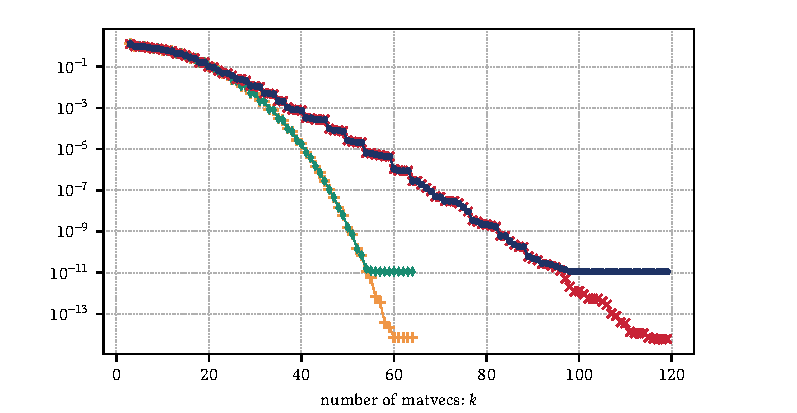
\includegraphics{imgs/ch6_sign_rat.pdf} 
    \end{center}
    \caption[{$\vec{A}^2$-norm error in Lanczos-OR-lm based rational approximation to matrix sign function.}]{%
    $\vec{A}^2$-norm error in Lanczos-OR-lm based rational approximation to matrix sign function.
    \hspace{.25em}\textit{Legend}:
    Lanczos-OR-lm based approximation of matrix sign function with
    ({\protect\raisebox{0mm}{\protect
\includegraphics[]{imgs/legend/l3.pdf}}})
    and without 
    ({\protect\raisebox{0mm}{\protect
\includegraphics[]{imgs/legend/l1.pdf}}}), 
    reorthogonalization.
    Lanczos-OR-lm based approximation of proxy rational matrix function with
    ({\protect\raisebox{0mm}{\protect
\includegraphics[]{imgs/legend/l4.pdf}}})
    and without 
    ({\protect\raisebox{0mm}{\protect
\includegraphics[]{imgs/legend/l2.pdf}}})
    reorthogonalization
    \hspace{.25em}\textit{Takeaway}: Lanczos-OR-lm can be applied to each term of a proxy rational function approximation of the sign function.
    }
    \label{fig:ch6_sign_rat}
\end{figure}


At least while while the application error for the Lanczos-OR approximation to the proxy rational matrix function is large relative to the approximation error, then as seen in \cref{eqn:triangle_ineq}, the error in approximating the matrix sign function is similar to the error in approximating the proxy rational matrix function.
However, as seen in \cref{eqn:reverse_triangle_ineq}, the final accuracy of approximating the matrix sign function is limited by the quality of the scalar approximation.

We also note that it really only makes sense to use Lanczos-OR-lm with a short-recurrence version of Lanczos, in which case the effects of a perturbed Lanczos recurrence are prevalent. 
In particular, as we noted in \cref{chap:intro} and discuss in detail in \cref{chap:finite_precision}, the algorithm encounters a delay of convergence as compared to what would happen with reorthogonalization.


\subsection{Lanczos-FA vs Lanczos-OR vs CG}
\label{ex:lanczos_msCG_comparison}

%
%All three approaches are use a rational function approximation to $f$, and we will 

%If the matrix $(a_i\vec{A}^2 + b_i \vec{A} + c_i \vec{I})$ is positive definite, as is often the case, then $\vec{x}_i = (a_i\vec{A}^2 + b_i \vec{A} + c_i \vec{I})^{-1} \vec{v}$ can be approximated using CG.


We now illustrate the effectiveness of the Lanczos-OR based approach to approximating rational matrix functions described in \cref{sec:rational_func}.
Then we compare an existing low-memory approach, called multishift CG, to the analogous approaches based on Lanczos-OR-lm and Lanczos-FA-lm.

Throughout this example, we will assume that $r$ is a rational function of the form
\begin{align}
\label{eqn:rat_form}
r = \sum_{i=1}^{m} \frac{A_ix^2+B_ix+C_i}{a_ix^2+b_ix+c_i}.
\end{align}
so that $r(\vec{A})\vec{b}$ has the form
\begin{align*}
    r(\vec{A})\vec{b} = \sum_{i=1}^{m} (A_i\vec{A}^2 + B_i\vec{A} + C_i\vec{I}) \vec{x}_i,
\end{align*}
where $\vec{x}_i$ is obtained by solving the linear system of equations $(a_i\vec{A}^2 + b_i \vec{A} + c_i \vec{I}) \vec{x}_i = \vec{b}$.
This is relatively general since any real valued rational function $r:\R\to\R$ with numerator degree smaller than denominator degree and only simple poles can be written in this form (in fact, this would be true even if $A_i=0$).
A range of rational functions of this form appear naturally; for instance by a quadrature approximation to a Cauchy integral formula representation of $f$ \cite{hale_higham_trefethen_08}.
Similar rational functions are seen in \cite{eshof_frommer_lippert_schilling_van_der_vorst_02,frommer_simoncini_09} and in the rational approximation tot the sign function given described in \cref{eqn:rational_func}.


In certain cases, the shift invariance of Krylov subspace can be used to simultaneously compute all of the $\vec{x}_i$ using the same number of matrix-vector products as would be required to approximate a single $\vec{x}_i$.
Specifically, suppose $(a_i\vec{A}^2 + b_i \vec{A} + c_i \vec{I})^{-1} \vec{v}$ can be written as $\vec{B}+z_i \vec{I}$ for all $i=1,\ldots, m$.
Then $\mathcal{K}_k(\vec{B}-z_i\vec{I},\vec{v})) = \mathcal{K}_k(\vec{B},\vec{v})$, so by constructing a single Krylov subspace $\mathcal{K}_k(\vec{B},\vec{v})$, one can compute all of the $\vec{x}_i$ and therefore $r\A\vec{v}$.
The resulting algorithms are typically called multishift-CG or multishift-MINRES \cite{eshof_frommer_lippert_schilling_van_der_vorst_02,frommer_simoncini_08,frommer_simoncini_08,guttel_schweitzer_21,pleiss_jankowiak_eriksson_damle_gardner_20}.
However, such an approach only works when $a_i = 0$ or $a_i = a$ and $b_i = b$, and in the latter case, matrix-vector products with $\vec{B}$ require two matrix-vector products with $\vec{A}$ and convergence depends only on the properties of $\vec{A}^2$ rather than $\vec{A}$.

Instead, we might apply Lanczos-FA-lm to compute individual terms of $r\A\vec{v}$.
However, if $(a_i\vec{A}^2 + b_i \vec{A} + c_i \vec{I})$ is indefinite, then Lanczos-FA may exhibit oscillatory behavior due to eigenvalues of $(a_i\vec{T}^2 + b_i \vec{T} + c_i \vec{I})$ near zero.
This may result in a breakdown of Lanczos-FA-lm similar to the breakdown which may be encountered by standard implementations of CG on indefinite linear systems.
Lanczos-OR-lm avoids such issues.

To highlight some of the tradeoffs between the algorithms, we construct several test problems by placing eigenvalues uniformly throughout the specified intervals.
In all cases, $\vec{v}$ has uniform weight onto each eigencomponent.
The outputs are computed using standard Lanczos, but we note that the spectrum and number of iterations are such that the behavior is quite similar to if full reorthgonalization were used. 
In particular, orthogonality is not lost since no Ritz value converges. 
The results of our experiments are shown in \cref{fig:msCG_squared}.

\begin{figure}[htb]
    \centering
    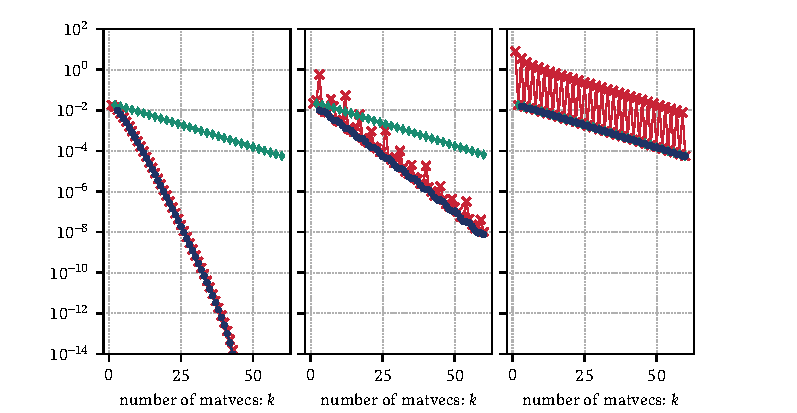
\includegraphics[]{imgs/ch6_lanczos_msCG_squared.pdf}
    \caption[{Comparison of $(\vec{A}^2+c\vec{I})$-norm errors for CG and Lanczos-FA for computing $(\vec{A}^{2}+c\vec{I})^{-1}\vec{v}$ with \( c=0.05 \).}]{%  
    Comparison of $(\vec{A}^2+c\vec{I})$-norm errors for CG and Lanczos-FA for computing $(\vec{A}^{2}+c\vec{I})^{-1}\vec{v}$ with \( c=0.05 \).  
    Here CG works with $\vec{A}^2+c\vec{I}$ and requires two matrix-vector products per iteration whereas Lanczos-FA works with $\vec{A}$ and requires just one.
    \hspace{.25em}\emph{Legend}: Lanczos-OR 
    ({\protect\raisebox{0mm}{\protect
\includegraphics[]{imgs/legend/l1.pdf}}}), 
    Lanczos-FA 
    ({\protect\raisebox{0mm}{\protect
\includegraphics[]{imgs/legend/l2.pdf}}}), and
    CG on squared system 
    ({\protect\raisebox{0mm}{\protect
\includegraphics[]{imgs/legend/l3.pdf}}}). 
    \hspace{.5em}
    \emph{Left}: eigenvalues on $[1,10]$. 
    \emph{Middle}: eigenvalues on $[-1.5,-1]\cup[1,10]$.
    \emph{Right}: eigenvalues on $[-10,-1]\cup[1,10]$. 
    \hspace{.25em}\emph{Legend}: Optimal algorithms have many nice convegence properties.
    }
    \label{fig:msCG_squared}
\end{figure}

We consider approximations to $r = 1/(x^2+0.05)$ with eigenvalues spaced with increments of $0.005$ throughout $[1,10]$, $[-1.5,-1]\cup[1,10]$, and $[-10,-1]\cup[1,10]$ respectively.
For each  example, the condition number of $\vec{A}^2+0.05\vec{I}$ is roughly 100 and the eigenvalues of $\vec{A}^2+0.05 \vec{I}$ fill out the interval $[1,100.05]$.
As such we observe that multishift CG converges at a rate (in terms of matrix products with $\vec{A}$) of roughly $\exp(-k/\sqrt{\kappa(\vec{A}^2)}) = \exp(-k/\sqrt{100})$ on all of the examples.

In the first example, $\vec{A}$ is positive definite.
Here Lanczos-FA and Lanczos-OR converge similarly to CG on $\vec{A}$ at a rate of roughly $\exp(-2k/\sqrt{10})$, where $k$ is the number of matrix-vector products with $\vec{A}$.

In the next example $\vec{A}$ is indefinite.
The convergence of CG is unchanged, because CG acts on $\vec{A}^2 + c\vec{I}$, it is unable to ``see'' the asymmetry in the eigenvalues of $\vec{A}$.
While the convergence of Lanczos-FA and Lanczos-OR is slowed considerably, both methods converges more quickly than CG due to the asymmetry in the intervals to the left and the right of the origin.
The convergence of these methods is at a rate of roughly $\exp(-k/\sqrt{15})$, although the exact rate is more complicated to compute \cite{fischer_96,schiefermayr_11}.
We also note the the emergence of oscillations in the error curve of Lanczos-FA.

In the third example, the asymmetry in the eigenvalue distribution about the origin is removed, and Lanczos-FA and Lanczos-OR converge at a rate very similar to that of multishift CG.
Note that Lanczos-FA displays larger oscillations, since the symmetry of the eigenvalue distribution of $\vec{A}$ ensures that $\vec{T}$ has an eigenvalue at zero whenever $k$ is odd.
However, the size of the oscillations is regularized by the fact that $c>0$.



